\section{\ix Design Approach}
\label{sec:design}

% We now present the fundamental design principles of a dataplane
% architecture designed to run untrusted, event-driven applicatxions, and
% designed to address the specific scalability challenges of today's
% web-scale applications.

The first three requirements of \S\ref{sec:motivation:challenges} --
high packet rate, microsecond latency, and connection scalability--
are not unique to event-driven, web-scale applications.  These
requirements are reasonably well understood and have been addressed in
the design of middleboxes such as firewalls,
load-balancers, and software
routers~\cite{DBLP:journals/tocs/KohlerMCJK00,DBLP:conf/sosp/DobrescuEACFIKMR09, missing-loadbalancers};
by integrating the networking stack and the application into a single
\emph{dataplane}. The two remaining requirements -- resource elasticity
and protection -- are not addressed in middleboxes because they
are single-purpose systems, not exposed directly to users.

% As for the other two remaining aspects -- resource elasticity and
% security and protection --, middleboxes provide fewer insights: since
% each middlebox typically performs a single function, resource
% elasticity and proportionality is less of a direct concern.  They are
% traditionally deployed and maintained using an embedded paradigm in
% which the entire stack -- operating system, applications and utilities
% -- is packaged as single blob.  As such, the security and protection
% model is not directly exposed to users.

Dataplanes differ from traditional OS designs in two fundamental
ways. First, they are designed to \emph{run each packet to
  completion}. All network protocol and application processing for a
packet is done before moving on to the next packet.  In contrast, a
commodity OS decouples protocol processing from the application itself
in order to enable flexibility in terms of resource scheduling and
flow control. For example, a commodity OS relies on device and soft
interrupts, to context switch from application processing to protocol
processing. Similarly, the kernel' networking stack will generate a
TCP \texttt{ACK} and slide its receive window even though the
application is not consuming data, up to some extent. Second,
dataplanes are designed to operate in a \emph{flow-consistent,
  coherence-free} manner.  Network flows are distributed into distinct
queues via receive-side scaling
(RSS)~\cite{DBLP:journals/computer/RegnierMIIMHNCF04}, so that the
common case processing of a packet requires no synchronization or
cache coherence interactions between cores.

% Flow-consistency distributes flows
% into distinct queues based on a L4-hash; this is routinely supported
% in network CPUs used in middleboxes (e.g., ~\cite{cavium-octeon}) as
% well as commodity NIC via Receive Side Scaling (RSS)~\cite{missing}.

Building upon the lessons from middleboxes, we design \ix to answer
the following question: {\it can the dataplane architecture be
  efficiently extended to support untrusted, event-driven applications
  and satisfy simultaneously the five requirements of
  \S\ref{sec:motivation:challenges}?}  The answer relies on the
following key design principles:


\myparagraph{Separation and protection of control and data plane:} 
% Software dataplanes are designed to operate on flows, not to
% provision resources or manage them in an elastic and proportional
% manner.
Our design separates the control function, responsible for resource
configuration, provisioning, scheduling, and monitoring, from the
dataplane, which runs the networking stack and application logic.
Like a conventional OS, the control plane multiplexes and schedules
resources among dataplanes but in an coarse-grain manner in space and
time: cores are dedicated to applications until revoked, memory is
allocated at large page granularity of physical memory; hardware queues are
exclusively assigned to a single dataplane until explicitly revoked.
Each dataplane runs a single application in a single address space.
This is similar to the Exokernel approach of using library operating
systems~\cite{DBLP:conf/sosp/EnglerKO95}, but with the additional
protection between applications and the control plane using the
ubiquitously available virtualization support in modern
servers~\cite{DBLP:journals/computer/UhligNRSMABKLS05,belay2012dune}.

\myparagraph{Native zero-copy API with explicit flow control:} We do
not expose or emulate the POSIX API for networking.  Instead, the
dataplane and the application communicate asynchronously with each
other via messages stored in
memory~\cite{rizzo2012netmap,han2012megapipe}.  The API meets the
commutativity rule~\cite{DBLP:conf/sosp/ClementsKZMK13} and allows for
a true zero-copy operation in both receive and transfer
directions. The dataplane and the application cooperatively manage the
message buffer pool. Incoming packets are mapped read-only into the
application that may hold onto message buffers and return them to the
dataplane at a later point.  The application sends to the dataplane
scatter/gather lists of memory locations for transmission but, since
the contents are not copied, the application must keep the content
immutable until the peer later acknowledges reception. The dataplane
implements all flow control mechanisms and may trim transmission
requests that exceed the available size of the sliding
window. However, since the dataplane does not introduce additional
buffering for outgoing packets, the application must make appropriate
policy decisions. Essentially, the API directly, but safely, exposes
flow control to applications.


% \myparagraph{Explicit flow control:} The API supports a zero-copy,
% non-blocking API that directly, but safely, exposes flow control to
% applications. The application may send to the dataplane scatter/gather
% lists of memory locations for transmission.  The kernel trims requests
% that exceed the available size of the sliding window. As the contents
% are not copied, the application must further keep the content
% immutable until the peer later acknowledges reception.  Although the
% kernel implements all flow control mechanisms, it does not introduce
% additional buffering or abstraction mechanisms, allowing applications
% to make appropriate policy decisions.


\myparagraph{Run to completion with adaptive batching:} Our dataplane
runs to completion all pipeline stages needed to receive or transmit a
packet, intermixing protocol processing (kernel mode) and application
logic (user mode) as needed. Hence, there is no need for intermediate
buffering between pipeline stages or between the application logic and
the TCP/IP stack. Batch processing minimizes instruction overheads and
increases cache locality.  Unlike previous proposals that batch only
at the API level in order to amortize system call
overhead~\cite{jeong2014mtcp,han2012megapipe}, we execute every
pipeline stage on a small batch of packets or commands in order to
fully amortize instruction caching effects and the overhead of PCIe
transfers.  To minimize the impact on latency, and improve utilization
on the outgoing wire, we adaptively batch and only in the presence of
congestion. We experimentally find that bounding batches to 128
packets is sufficient to amortize all noticeable per-packet overheads.

% Christos; this is essentially the other half of the "expose flow
% control to applications". oh well...
The combination of adaptive batch processing and zero copy means that
queues for incoming packets can build up only at the NIC edge, before
packets are processed by the dataplane. The networking stack sends
acknowledgments to peers only as fast as the application can process
them. Any slowdown in the application-processing rate quickly leads to
shrinking windows in peers. We can also monitor the monitor queue
depths at the NIC edge and signal the control plane to allocate
additional resources for the dataplane (more hardware threads,
increase clock frequency), notify peers explicitly about congestion
(e.g., via ECN~\cite{ramakrishnan2001addition}), and finally make
policy decisions for congestion management (e.g., via
RED~\cite{DBLP:journals/ton/FloydJ93}).

% \myparagraph{Buffering at the NIC edge:} The consequence of adaptive
% batching is the buildup of queues at the NIC edge before the packets
% are processed by the dataplane.  Because of the dataplane's design,
% congestion occurs only at the NIC edge.  In effect, the NIC edge acts
% like the last-hop buffer in the network.  This has an additional
% benefit in terms of flow control, as the networking stack sends
% acknowledgments to peers only as fast as the application can process
% them.  Congestion in the NIC edge therefore leads to shrinking windows
% in peers, and flow control.


% Like switches and routers, the NIC edge can
% monitor queue depths to detect congestion, signal the control plane to
% allocate additional resources (more hardware threads, increase clock
% frequency) for the dataplane, notify explicitly flow sources of
% congestion (e.g., via ECN~\cite{ramakrishnan2001addition}), and finally make
% policy decisions when it is necessary to manage congestion (e.g., via RED~\cite{DBLP:journals/ton/FloydJ93}).

\begin{figure}
\begin{centering}
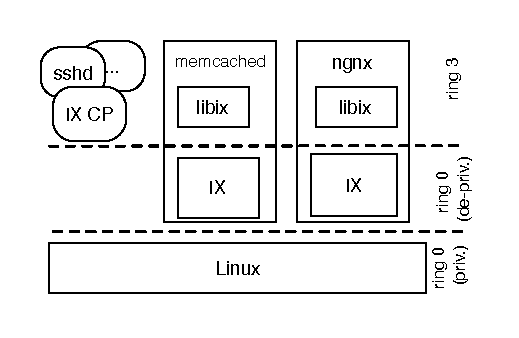
\includegraphics{figs/cp-dp.eps}
\centering\caption{Protection and separation in \ix.}
\label{fig:cp-dp}
\end{centering}
\end{figure}





\myparagraph{Flow consistent, coherence-free processing:} We use
multi-queue NICs with RSS support to provide flow-consistent hashing
of incoming traffic to distinct hardware queues. Each queue is served
by a single hardware thread all the way to the application layer,
eliminating the need for synchronization and cache coherence traffic
between cores. Similarly, memory management is organized in distinct
pools for each hardware thread. The absence of a socket layer
eliminates the issue of the shared file descriptor namespace in
multithreaded
applications~\cite{DBLP:conf/sosp/ClementsKZMK13}. Hence, our design
scales well with the increasing number of cores in modern servers. Our
approach does not restrict the memory model for
applications. Application logic can take advantage of coherent, shared
memory to exchange information and synchronize between cores.




